\section{Estatísticas Gerais}

Nesta seção, apresentamos as estatísticas gerais dos dados coletados para os dispositivos Smart TV e Chromecast. As análises incluem cálculos de medidas descritivas, como média, variância e desvio padrão, além de representações gráficas através de histogramas, boxplots e funções de distribuição empírica (ECDF). 

\subsection{Medidas Descritivas}

As medidas descritivas para as taxas de upload e download (em escala logarítmica base 10) estão resumidas na Tabela~\ref{tab:estatisticas}. 

\begin{table}[H]
\centering
\caption{Medidas descritivas das taxas de upload e download.}
\label{tab:estatisticas}
\begin{tabular}{|c|c|c|c|c|}
\hline
\textbf{Dispositivo} & \textbf{Tipo de Tráfego} & \textbf{Média} & \textbf{Variância} & \textbf{Desvio Padrão} \\ \hline
Smart TV & Upload & 2.16 & 4.11 & 2.03 \\ \hline
Smart TV & Download & 2.35 & 6.72 & 2.59 \\ \hline
Chromecast & Upload & 3.35 & 0.46 & 0.68 \\ \hline
Chromecast & Download & 3.80 & 1.66 & 1.29 \\ \hline
\end{tabular}
\end{table}

\subsection{Visualizações Gráficas}

Para compreender melhor a distribuição dos dados, utilizamos as seguintes representações gráficas:

\begin{itemize}
    \item \textbf{Histogramas:} As distribuições das taxas de upload e download para cada dispositivo estão representadas nos histogramas da Figura~\ref{fig:histogramas}.
    \item \textbf{Boxplots:} A Figura~\ref{fig:boxplots} mostra os boxplots comparando as taxas de upload e download entre Smart TV e Chromecast.
    \item \textbf{ECDF:} As funções de distribuição empírica, exibidas na Figura~\ref{fig:ecdf}, demonstram a probabilidade acumulada para cada valor das taxas.
\end{itemize}

Para a construção dos histogramas, o número de bins foi calculado utilizando o método de Sturges:

\begin{equation}
k = 1 + \log_2(n),
\end{equation}

onde \(n\) é o número total de amostras. Este método busca otimizar a visualização dos dados ao balancear granularidade e clareza.

O número de bins calculado para cada dispositivo é o seguinte:
\begin{itemize}
    \item \textbf{Smart TV:} \(k = 24\) bins.
    \item \textbf{Chromecast:} \(k = 22\) bins.
\end{itemize}

\begin{figure}[H]
    \centering
    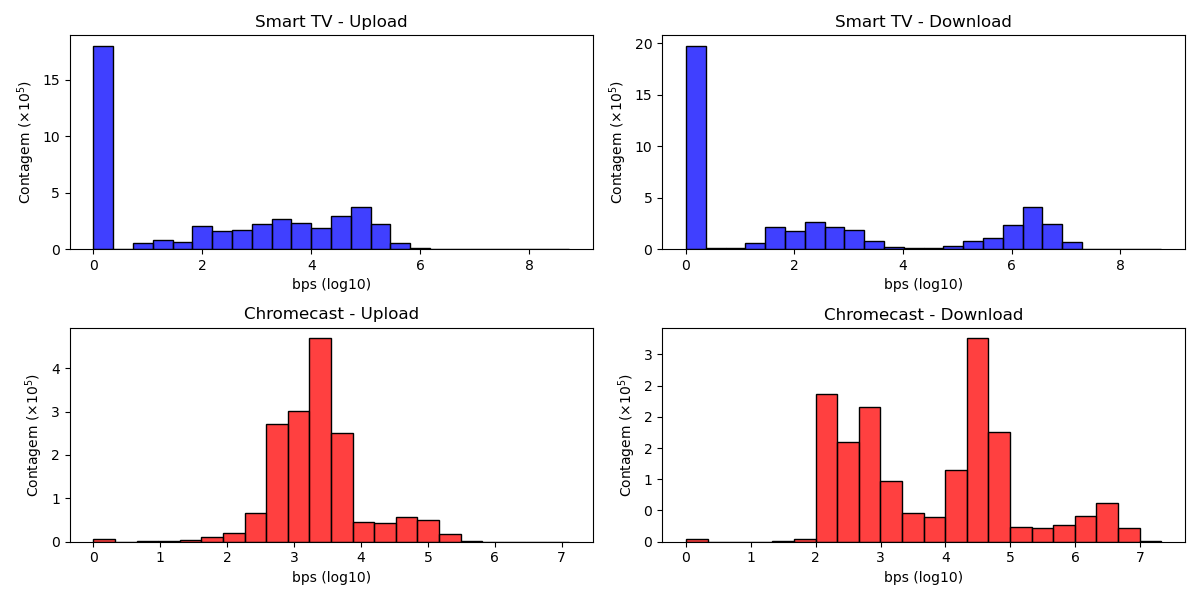
\includegraphics[width=0.8\textwidth]{../estatísticas gerais/histogramas.png}
    \caption{Histogramas das taxas de upload e download para Smart TV e Chromecast.}
    \label{fig:histogramas}
\end{figure}

\begin{figure}[H]
    \centering
    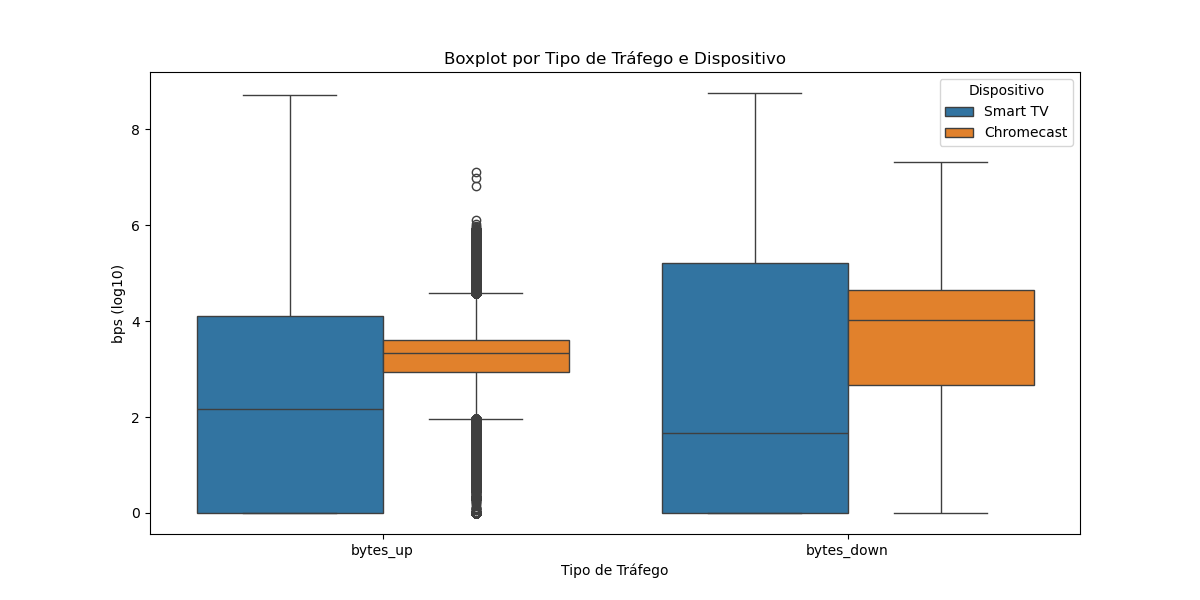
\includegraphics[width=0.8\textwidth]{../estatísticas gerais/boxplot.png}
    \caption{Boxplots das taxas de upload e download para Smart TV e Chromecast.}
    \label{fig:boxplots}
\end{figure}

\begin{figure}[H]
    \centering
    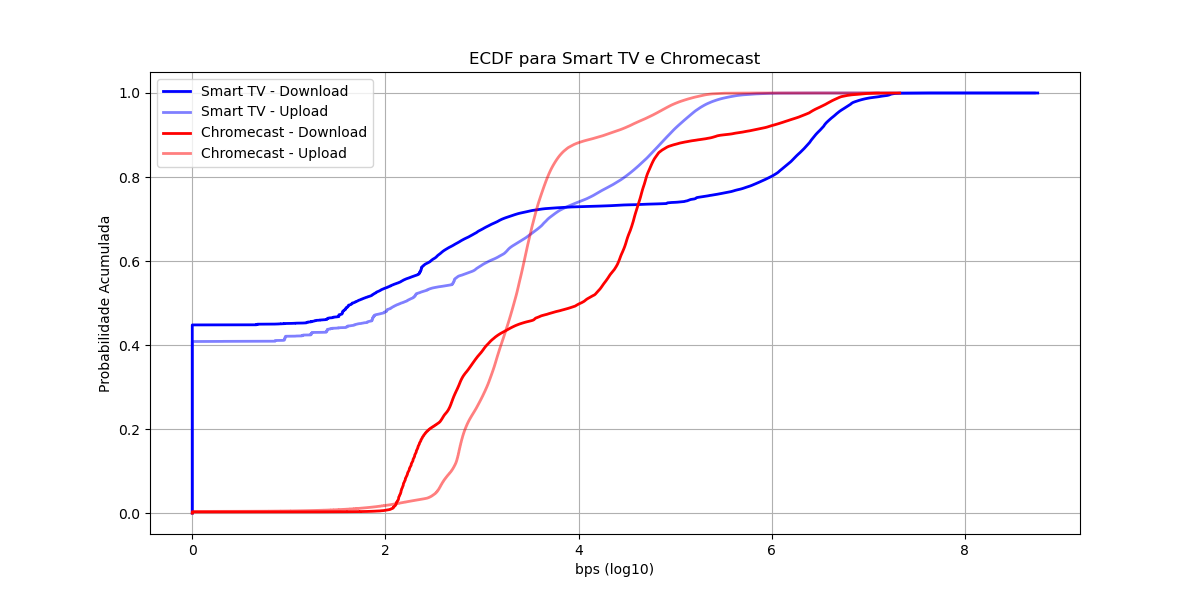
\includegraphics[width=0.8\textwidth]{../estatísticas gerais/ecdf.png}
    \caption{Funções de Distribuição Empírica (ECDF) das taxas de upload e download.}
    \label{fig:ecdf}
\end{figure}

\subsection{Análise dos Resultados}

Os resultados destacam diferenças importantes nas características das taxas de upload e download entre os dispositivos Smart TV e Chromecast.

\begin{itemize}

\item \textbf{Smart TV:} 
As taxas de upload e download da Smart TV possuem médias parecidas e variâncias relativamente altas, indicando uma dispersão maior dos dados. As taxas estão predominantemente concentradas em valores baixos, especialmente em valores iguais a zero, conforme já havia sido evidenciado na Análise Exploratória dos Dados (Seção~\ref{sec:eda}). Essa característica é refletida na primeira barra dos histogramas (Figura~\ref{fig:histogramas}), que é consideravelmente maior do que as demais. No boxplot (Figura~\ref{fig:boxplots}), essa concentração é representada pela proximidade do limite inferior ao primeiro quartil (\( Q1 \)). Na mesma figura também, é possível observar a ausência de outliers nos dois tipos de tráfego. Além disso, a ECDF (Figura~\ref{fig:ecdf}) apresenta um valor inicial relativamente alto, superior a 0.4, devido à grande quantidade de valores nulos, crescendo de forma lenta até chegar ao valor máximo.

\item \textbf{Chromecast:} 
As taxas de upload e download do Chromecast também possuem médias próximas, mas apresentam desvios padrão relativamente baixos, indicando uma dispersão menor dos dados. A taxa de download (\texttt{bytes\_down}) exibe uma variância maior do que a de upload (\texttt{bytes\_up}). A taxa de upload apresenta muitos outliers, tanto para valores altos (picos) quanto para valores baixos (vales), como destacado no boxplot (Figura~\ref{fig:boxplots}), enquanto a taxa de download não possui nenhum. A ECDF (Figura~\ref{fig:ecdf}) reflete essa característica, apresentando um crescimento rápido após \(10^2\) bps.

\item \textbf{Comparação Geral:} A Smart TV e o Chromecast apresentam diferenças marcantes em seus padrões de tráfego. Enquanto a Smart TV concentra grande parte de seus dados em valores baixos, com ausência de outliers, o Chromecast exibe menor dispersão geral, mas com muitos outliers na taxa de upload. A ECDF da Smart TV cresce de forma lenta devido aos valores nulos iniciais, enquanto a do Chromecast apresenta um crescimento rápido após \(10^2\) bps, refletindo uma concentração maior em valores intermediários. Essas diferenças sugerem que a Smart TV alterna entre períodos de inatividade e altos fluxos, enquanto o Chromecast apresenta tráfego mais estável, mas com picos e vales ocasionais no upload.

\end{itemize}Essas observações podem auxiliar no desenvolvimento de estratégias de gerenciamento de rede mais eficientes, considerando a alta variabilidade e períodos de inatividade da Smart TV, e os picos de tráfego ocasionais no upload do Chromecast. Adaptar essas estratégias às características específicas de cada dispositivo pode melhorar a alocação de recursos e a experiência do usuário.